\documentclass[notas.tex]{subfiles}

\begin{document}
\chapter{Geometry dependence of quantum Hall wave functions} \label{sec_geometry_dependence}

\section{Introduction to the QHE} \label{sec_intro_qhe} 

Here, we present a brief physical overview of the \emph{QHE (quantum Hall effect)}. For references on this topic see, for instance, \cite{jain_composite_2007, yoshioka_quantum_2002}.

The QHE is the name given to the behaviour shown by the Hall resistivity $\rho_{xy}$ and the longitudinal resistivity $\rho_{xx}$ of electron systems as a strong transversal magnetic field varies. In this overview, we will focus on the case of the plane, the simplest and first geometry where the QHE was studied. 

When considering the quantum Hamiltonian for quantum Hall systems, its eigenvalues (i.e. the energy levels) are commonly referred to as \emph{Landau levels}. Landau levels are, in most cases, degenerate (i.e. the dimension of the corresponding eigenspace is greater than one). Of special relevance is the \emph{LLL (lowest Landau level)}, i.e. the lowest energy level. 

The most interesting quantity is the Hall resistivity, expressed as
\begin{align*}
	\rho_{xy} = \frac{2 \pi \hbar}{e^2} \frac{1}{\nu},
\end{align*}
where $\nu$ is a parameter, called the \emph{filling fraction}, which varies with the magnetic field $B$, $-e$ is the charge of an electron and $\hbar$ is the reduced Planck's constant. In the \emph{IQHE (integer quantum Hall effect)}, the Hall resistivity varies in discrete jumps $\nu \in \ints$. The longitudinal resistivity $\rho_{xx}$, on the other hand, vanishes, spiking only when $\rho_{xy}$ jumps to the next plateau. As disorder decreases, we obtain the \emph{FQHE (fractional quantum Hall effect)}, where $\nu \in \rats$ can take rational values. 

 %In what follows, we are omit the magnetic length $l_B = \sqrt{\frac{\hbar}{eB}}$ and we do not normalize the wave functions. 
 One basis for the LLL eigenspace in the plane for the one-particle case, which shows its degeneracy, is
\begin{equation} \label{eq_single_wavefunction}
	\psi_m \sim z^m e^{- \frac{\abs{z}^2}{4}}, m \in \nats_0.
\end{equation}

We now present the ground state wave functions for multiple particles in the lowest Landau level, both in the case of the IQHE and of the FQHE. We will denote the number of particles in the system by $N \in \nats$. 

In the IQHE, the number of particles is such that the LLL is fully filled, and we can assume that the electrons are non-interacting. We can thus obtain the wave function for the fully filled lowest Landau level in the multi-particle Hilbert space using the \emph{Slater determinant}
\begin{align*}
	\psi_{IQHE} &\sim \begin{vmatrix}
		\psi_1(z_1) & \hdots & \psi_1(z_N) \\
		\vdots & \ddots & \vdots \\
		\psi_N(z_1) & \hdots & \psi_N(z_N)
	\end{vmatrix} e^{-\frac{\sum_{k=1}^N \abs{z_k}^2}{4}}
\end{align*}
which, substituting by the $\psi_i, i \in \{1,...,N\}$ in \eqref{eq_single_wavefunction}, yields the \emph{Vandermonde determinant}
\begin{align} \label{eq_integer_wavefunction}
	\psi_{IQHE} &\sim \begin{vmatrix}
		z_1^0 & \hdots & z_N^0 \\
		\vdots & \ddots & \vdots \\
		z_1^{N-1} & \hdots & z_N^{N-1}
	\end{vmatrix} e^{-\frac{\sum_{i=1}^N \abs{z_i}^2}{4}} \nonumber \\ 
	&= \prod_{1 \leq k<j \leq N}(z_k - z_j) e^{-\frac{\sum_{k=1}^N \abs{z_k}^2}{4}}.
\end{align}

In the fractional quantum Hall effect, the LLL is only partially filled. This makes it so that the interaction between electrons must be taken into account, which in turn makes the problem of obtaining an exact expression for the ground state wave function essentially intractable. A solution to this, employed by Laughlin, is to write an approximate wave function based on an ansatz \cite{laughlin_anomalous_1983}. This wave function, the \emph{Laughlin wave function} (or \emph{Laughlin state}), is valid for filling fractions $\frac{1}{m}$, with $m$ odd. For $N$ electrons, it takes the form
\begin{align} \label{eq_laughlin_wavefunction}
	\psi_\text{L} \sim \prod_{1 \leq k < j \leq N}(z_k - z_j)^m e^{\frac{-\sum_{k=1}^N \abs{z_k}^2}{4}}.
\end{align}
We may also consider quasiholes which, physically, carry a fraction of the absolute value of the charge of the electron. For $R$ quasiholes at $\nu_1,...,\nu_R$, the wave function takes the form
\begin{align} \label{eq_laughlin_wavefunction_qh}
	\psi_\text{L,QH} \sim \prod_{j = 1}^{N}\prod_{k = 1}^{R}(z_j - \nu_k) \prod_{1 \leq k < j \leq N}(z_k - z_j)^m e^{\frac{-\sum_{k=1}^N \abs{z_k}^2}{4}}.
\end{align}
For filling fractions $\frac{1}{m}$, with $m$ even, the above expressions are clearly no longer valid (one can see that the wave function no longer displays fermionic exchange statistics). To describe the lowest Landau level in this case, we must instead consider the \emph{Moore-Read wave function} (or \emph{Moore-Read state}), first introduced by Moore and Read in \cite{moore_nonabelions_1991}. For an even number of electrons, it takes the form
\begin{align}\label{eq_mr_wavefunction}
	\psi_{\text{MR}} \sim \Pf\left ( \frac{1}{z_i - z_j} \right ) \prod_{1 \leq k < j \leq N}(z_k - z_j)^m e^{\frac{-\sum_{k=1}^N \abs{z_k}^2}{4}},
\end{align}
where, for $M$ an even-dimensional matrix, $\Pf(M)$ is the \emph{Pfaffian} of $M$ and is defined by the property $\Pf^2(M) := \det(M)$. 
% We will also consider quasiholes, which are local excitations of the quantum Hall system. These carry an electric charge of $\frac{e}{m}$, a fraction of the electric charge of an electron. The Moore-Read wave function with $n$ electrons and $r$ quasiholes takes the form
% \begin{align} \label{mr_wavefunction_qh}
% \Psi_{\text{MR}} = \Pf\left ( \frac{1}{z_i - z_j} \right ) \prod_{j = 1}^{n}\prod_{k = 1}^{r}(z_j - \nu_k) \prod_{j > k}^n(z_j - z_k)^m e^{\frac{-\sum_i \abs{z_i}^2}{4 l_B^2}}.
% \end{align}

\section{Dynamics of a particle on a magnetic field} \label{sec_gq_particle_magnetic} In this section, we quickly summarize the dynamics of a charged particle on a Riemannian manifold under the action of a magnetic field. We  base ourselves on \cite{tejero_prieto_holomorphic_2006}. 

Let $(\nfld, \metric)$ be the Riemannian manifold on which the particle is moving. The magnetic field is represented by a differential $2$-form $F \in \dform^2(\nfld)$, which we will assume to be closed and nondegenerate, and the motion is described on the symplectic manifold
\begin{align*}
	(\mfld = T^*\nfld, \sform = d\spot + e \pi^* F),
\end{align*}
where $e$ is the electric charge of the particle, $\pi: T^*\nfld \to \nfld$ is the projection to the base manifold and $\spot$ is the tautological form on $T^*\nfld$. The dynamics on $T^*\nfld$ is described by the Hamiltonian
\begin{align*}
	H: T^*\nfld &\to \reals\\
	\alpha &\mapsto \frac{1}{2}\frac{\norm{\alpha^{\sharp_\gamma}}_\metric^2}{m},
\end{align*}
where $m$ is the mass of the particle and $\norm{\cdot}_\metric := \metric(\cdot, \cdot)^\frac{1}{2}$.

Since $d\spot$ is exact,
\begin{align*}
	\left[ d\spot + e \pi^* F \right ] \in H^2(T^*\mfld, \ints) \iff [ e F ] \in H^2(\mfld, \ints),
\end{align*}
which implies that
\begin{prop} \label{prop_magnetic_sform}
	Let $F \in \dform^2(\nfld)$ be a closed, non-degenerate differential $2$-form on $\nfld$. Then, the symplectic manifold $(T^*\nfld, \sform = d\spot + e \pi^* F)$ is quantizable if and only if the symplectic manifold $(\nfld, eF)$ is quantizable.
\end{prop}

From the previous remarks, we see that a prequantization bundle on $(T^*\nfld, \sform)$ is equivalent to the pullback of a prequantization bundle on $(\nfld, eF)$.  Because of this, the latter are also called prequantization line bundles on $(T^*\mfld, \sform)$ and will be the ones under consideration in the following sections.

\begin{rem} \label{rem_effective_geometry}
	In what follows, we will impose an additional restriction on the form $eF$ besides asking that $(\nfld, eF)$ is quantizable. Assuming that $\nfld$ is a Riemann surface (i.e. a complex manifold in one complex dimension) with complex structure $\cstruct$, we ask that $(eF, \metric, \cstruct)$ forms a Kähler triple, which endows $\nfld$ with an \emph{effective Kähler geometry}.
\end{rem}

\section{Evolution of quantum Hall ground states} \label{sec_geometry_dependence_overview}
In this section, we bring together the theory developed in \secref{sec_prelim} in order to determine how the quantum Hall wave functions change as the Riemann surface $\nfld$ associated to the quantum Hall system is deformed. 

We will be working with an effective geometry as in \remref{rem_effective_geometry} and, by abuse of notation, we assume that $\sform = eF$ represents the magnetic field on $\nfld$, and not the symplectic form on $T^*\nfld$ as in \secref{sec_gq_particle_magnetic}. In this effective geometry, the quantum Hall states for the LLL are actually holomorphic sections of a prequantization of $(\nfld^N, \sum_{j=1}^{N} \sform_j)$, and take the form given in \propref{prop_polarized_holo_sections}, as will be clear from the examples.

In all examples, the general procedure is similar and is outlined below. 

\begin{enumerate}
	\item Fix a Riemann surface $\nfld$ with Kähler pair $( \sform, \cstruct_0)$.
	\item Define a Hamiltonian $S^1$-action $\tact: S^1 \times \nfld \to \nfld$ as in \defref{def_ktoric_action} and write the corresponding moment map $\mmap: \nfld \to \reals$.
	\item Write down action-angle coordinates $(u, \theta)$ as in \eqref{eq_aa_coords} and toric holomorphic coordinates $v+i\theta$ as in \eqref{eq_kt_coords} on $\nfld^\circ$. Pick an $S^1$-invariant Kähler potential $\kpot_0 \in C^\ra(\nfld^\circ)$ i.e. one depending only on the symplectic (momentum) coordinate $u$, and obtain an initial symplectic potential $\sgen_0$ using the Legendre transform \eqref{eq_legendre_transform}.
	\item Choose an $S^1$-invariant Hamiltonian $H \in C^\ra(\nfld)$, strictly convex in the variable $u$. $S^1$-invariance is imposed so that the calculations can be performed explicitly; strict convexity ensures that $(\sform, J_s)$ remains a Kähler pair, where $J_s = (\phi_{is})^* J_0$ and $\phi_{\tau}$ is the complex flow of $X_H$ (see e.g. \cite[Section 2.3]{baier_toric_2011}).
	\item Calculate the complex-time flow of $X_H = H' X_u = - H' \pd{\theta}$, $\phi_\tau$, as in \thmref{thm_complex_flow}, and use it to obtain the time-evolution of the toric holomorphic coordinates (and, thus, of the complex structure),
	\begin{align} \label{eq_cylinder_ktoric_evolution}
		\left ( \phi_\tau^{X_H} \right )^* (v+is) \big|_{\tau=is} = v + i(\theta - \tau H'(u)) \big|_{\tau=is} = v + sH' + i \theta = v_{s} + i \theta,
	\end{align}
	where $v_{s} := v + sH'$ and $'$ denotes the derivative with respect to $u$.
	\item \label{intro_symplectic_evolution} Assuming that the symplectic form and action-angle coordinates are kept fixed, determine the symplectic potential and its evolution $\sgen_s$ as in \eqref{eq_coordinate_change},
	\begin{align*}
		v_{s} = v + sH' = \ppd{\sgen_0}{u}(u) + sH'(u) = \ppd{\sgen_{s}}{u}(u).
	\end{align*}
	Integrating, we obtain
	\begin{align*}
		\sgen_{s} = \sgen_0 + sH.
	\end{align*}
	\item Use the time-evolved symplectic potential to determine the relevant geometric quantities
	\begin{align*}
		\metric_s &= \sgen_s'' du^2 + \frac{1}{\sgen_s''} d \theta^2, \\
		\kpot_s &= u\frac{\partial \sgen_s}{\partial u} - \sgen_s,  \\
		S_s &= - \left ( \frac{1}{\sgen_s^{''}} \right )''.
	\end{align*}
	where $\metric_s$ is the metric, $\kpot_s$ is the Kähler potential and $S_s$ is the scalar curvature, all at complex time $\tau=is$.
	\item Consider the configuration space for $N \in \nats$ particles as the Cartesian product $\nfld^N$ and take the Hamiltonian $\bm{H} = \sum_{k=1}^{N} H_k$, where $\pi_k: \nfld^N \to \nfld$ is the projection on the $k$th element of this Cartesian product and $H_k = \pi_k^*H$. Note that, on the Cartesian product, there is a corresponding toric action (and associated charts) and complex-time flow which are given by this Hamiltonian.
	
	Pick a prequantization, $(L, \hip{\cdot}{\cdot}, \covdsymb)$ and a unitary trivialization $\utriv$ on $\nfld^\circ$ (which is possible for the cases considered). Pick a square root $\sqrtb_{\pol_0}$ of the canonical bundle, where $\pol_0$ is the Kähler polarization (see \defref{def_kahler_polarization}) associated to the complex structure $\cstruct_0$ of $\nfld$. 
	\item \label{intro_operator_notation} Determine the prequantization and the quantization of the Hamiltonian $\bm{H}$ as in \eqref{eq_prq_whf} and \remref{rem_full_quantization} and write down the corresponding GCST as in \eqref{eq_cst_def}.
	\begin{align*}
		\prqhf{\bm{H}} &=  \prqs_1(\bm{H}) \otimes I +  I \otimes \prqs_2(\bm{H}) \\
		\prqs_{1}(\bm{H}) &= \sum_{k=1}^{N} \prq{H_k} = \sum_{k=1}^{N} - i  H_k'(u) \pd{\theta} - \spot \left( H_k'(u_k) \pd{\theta} \right) + H_k \\
		\prqs_{2}(\bm{H}) &= \sum_{k=1}^{N} i \lied{- H'(u) \pd{\theta_k}} \\
		\prq{u_k} &= - i  \pd{\theta_k} \\
		\q{\bm{H}} &=  \qs_1 \otimes I +  I \otimes \qs_2 \\
		\qs_1(\bm{H}) &= \sum_{k=1}^{N} H_k(\prq{u_k}) = \sum_{k=1}^{N} H_k \left (- i  \pd{u_k} \right )  \\
		\qs_2(\bm{H}) &= \sum_{k=1}^{N} H_k \left (i\lied{-\pd{\theta_k}} \right ) = - \sum_{k=1}^{N} \frac{\left( \lied{-\pd{\theta_k}}\right)^2}{2}  \\
		U_s &= \left ( e^{-i \tau \prqhf{\bm{H}}} \circ e^{i \tau \q{\bm{H}}} \right )\big|_{\tau = is} \\
		&= U_{1,s} \circ U_{2,s} \\
		U_{j,s} &= \left ( e^{-i \tau \prqs_j(\bm{H})} \circ e^{i \tau \qs_j(\bm{H})} \right )\big|_{\tau = is}, \qquad j \in \{1,2\}.
	\end{align*}
	\item Apply the GCST to the quantum Hall states in order to determine how they evolve as the manifold is deformed.
\end{enumerate}

We will treat two cases: that of the plane and of the cylinder. For simplicity, throughout this section, we set $\hbar = 1$. 

\section{Evolution on a deformed plane with $S^1$-symmetry} \label{sec_plane}
In this section, our manifold will be $\reals^2$ with the standard symplectic structure and standard complex structure as the initial complex structure.

We will consider the Kähler toric action 
\begin{align*}
	\tact: S^1 \times \reals^2 &\to \reals^2 \\
	(e^{it}, (x, y)) &\mapsto (\cos (t) x - \sin(t) y, \sin(t) x + \cos(t) y) 
\end{align*}
given by rotations around the origin. This action has moment map
\begin{align*}
	\mmap: \reals^2 &\to \reals \\
	(x, y) &\mapsto \frac{x^2 + y^2}{2}.
\end{align*}
The open set where this action is free is $(\reals^2)^\circ = \reals^2 \setminus \{0\}$. Defining the coordinate $u = \mmap = \frac{x^2 + y^2}{2}$ on $P^\circ = (\image \mu)^\circ = \reals^+$ and taking the angular coordinate $\theta$ on $S^1$, then 
\begin{align*}
	\phi: \reals^+ \times S^1 &\to (\reals^2)^\circ \\
	(u, \theta) &\mapsto \left (\sqrt{2u} \cos \theta, \sqrt{2u} \sin \theta \right )
\end{align*}
define action-angle coordinates on $(\reals^2)^\circ$; indeed, note that in theese coordinates the toric action is represented by  $\hat \mmap(e^{it})(u, \theta) = (u, \theta + t)$. As expected, the symplectic form is written as
\begin{align*}
	dx \wedge dy = d (r \cos \theta) \wedge d(r \sin \theta) = r dr \wedge d \theta = d\left( \frac{r^2}{2} \right) \wedge d \theta = du \wedge d\theta,
\end{align*}
where $r$ is the usual radial coordinate. 

We consider the usual complex structure and the holomorphic chart 
\begin{align*}
	\zeta: \reals \times iS^1 &\to \cmplx^\circ \\
	v + i\theta &\mapsto e^{v + i\theta},
\end{align*}
where $\cmplx^\circ = \cmplx \setminus \{0\}$. Note that this chart is actually toric holomorphic since, in this chart, the action is represented by $\tilde \mmap(e^{it})(v + i\theta) = v + i(\theta + t)$. 

The initial toric holomorphic and action-angle coordinates are related as
\begin{align*}
	v = \frac{1}{2}\log(2u), \qquad	u = \frac{1}{2}e^{2v}.
\end{align*}
Choose the $S^1$-invariant Kähler potential $\kpot(v) = \frac{e^{2v}}{2} = \frac{u^2}{2}$ and obtain the initial symplectic potential through the Legendre transform as in \eqref{eq_legendre_transform}
\begin{align*}
	 \sgen_0(u) = \sum_{j} u \cdot v(u) - \kpot_0(v(u)) = \frac{u}{2}\log(2u) - \frac{u}{2}.
\end{align*}
From point \eqref{intro_symplectic_evolution}, we obtain
\begin{align*}
	\sgen_{s} = \frac{u}{2} \log(2u) - \frac{u}{2} + sH.
\end{align*}
We will take $H = \frac{u^2}{2}$ as our Hamiltonian. From this and the previous considerations we obtain
\begin{align} 
% g(u) &= \frac{u}{2}\log(2 u) - \frac{u}{2}, \nonumber \\
% g_s &= \frac{u}{2}\log(2 u) - \frac{u}{2} + s\frac{u^2}{2},  \nonumber \\
\kpot_s &= % ug' - g + s(uH' - H) = 
(su+1)\frac{u}{2},\label{eq_plane_kpot_evo} \\
\gamma_s % &= \left ( \frac{2sH''u+1}{2u} \right )du^2 + \left ( \frac{2sH''u+1}{2u} \right )^{-1} d \theta ^2, \\
&=  \left ( \frac{2su+1}{2u} \right )du^2 + \left ( \frac{2su+1}{2u} \right )^{-1} d \theta ^2, \\
S_s &= \frac{8s}{1+2su}. \label{eq_plane_curvature_evo}
\end{align}

\begin{figure}[htbp]
	\centering
	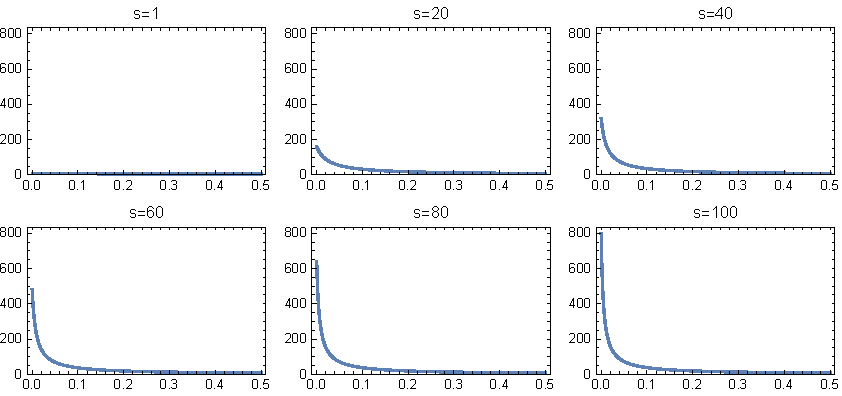
\includegraphics[width=1.0\textwidth]{plane_curvature.pdf}
	\caption{Curvature of plane \eqref{eq_plane_curvature_evo} plotted as a function of $u$.}
	\label{fig_plane_curvature}
\end{figure}
\begin{figure}[htbp]
	\centering
	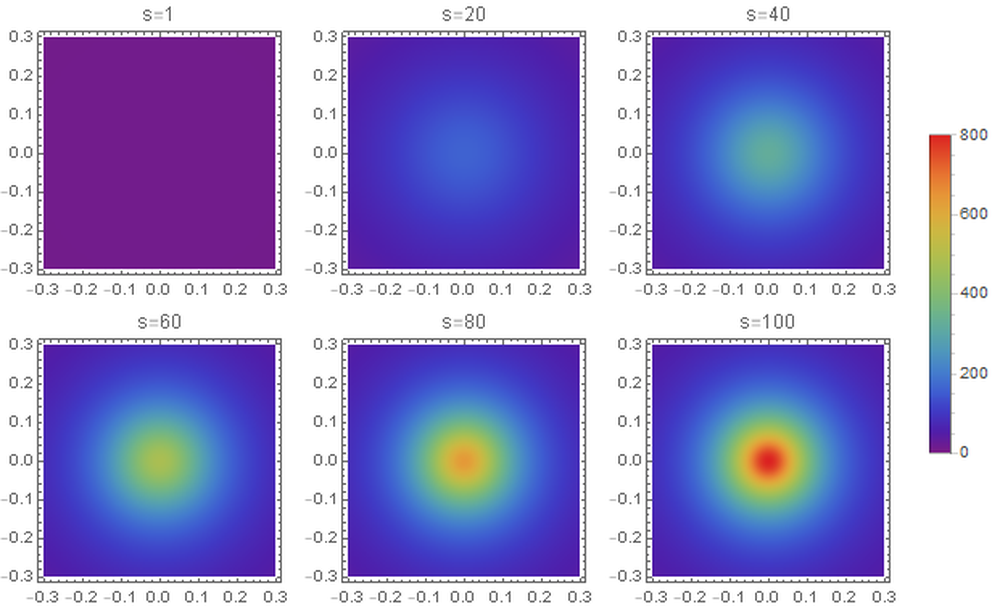
\includegraphics[width=1.0\textwidth]{sp_plane_curvature_density.png}
	\caption{Density plot of the curvature of the plane \eqref{eq_plane_curvature_evo} plotted as a function of $x$ and $y$.}
	\label{fig_plane_curvature_density}
\end{figure}



% The time-evolved complex coordinate is such that
% \begin{align} \label{eq_plane_normal_evolution}
% 	z_s := \left ( \phi_\tau^{X_H} \right )^* z \big|_{\tau=is} = e^{su}z
% \end{align}

Let us now extend this to $N \in \nats$ particles. The Riemann surface representing the configuration space of the particles will be the Cartesian product $(\reals^2)^N \cong \reals^{2N}$. We consider the trivial complex line bundle, $L = \reals^{2N} \times \cmplx$, with $\spot = \sum_{k=1}^{N} u_k d\theta_k$, unitary trivialization $\utriv \equiv 1$, connection $\covd{X} = X + i \spot(X)$ and Hermitian structure $\hip{a}{b} = a \bar b$ for $a, b \in C^\infty(\reals^{2n}; \cmplx)$. The square root $\sqrtb_\pol$ of the canonical bundle is trivial with trivializing section represented by $\sqrt{dz_1 \wedge ... \wedge dz_N}$. The polarization $\pol_0$ comes from the complex structure i.e. $\overline \pol_0$ is spanned by $\{\pd{\bar z_k}\}_{k=1,...N}$, and the time-evolved polarization $\pol_\tau$ is such that $\overline \pol_\tau$ is spanned by $\{\pd{(\bar z_{s})_k}\}_{k=1,...,N}$, where $(z_{s})_k = \left ( \phi_{\tau}^{X_H} \right )^* z_k \big|_{\tau=is}$ and $\bm{H} = \sum_{k=1}^{N} \frac{u_k^2}{2}$. 


 In order to write the GCST associated to $\bm{H}$, we first determine the prequantizations and quantizations of the relevant observables. We use the notation of point \eqref{intro_operator_notation}.
\begin{align}
\prqs_1(\bm{H}) &= \sum_{k=1}^{N} \left( - i  u_k\pd{\theta_k} - \frac{u_k^2}{2} \right), \nonumber\\
\prqs_2(\bm{H}) &= i \sum_{k=1}^{N} \lied{\left( - u_k \pd{\theta_k} \right)}, \nonumber\\
% \prqhf{\bm{H}} &= \sum_{k=1}^{n} \left[ \left( - i  u_k\pd{\theta_k} - \frac{u_k^2}{2} \right) \otimes I + i   I \otimes \lied{- u_k \pd{\theta_k}} \right] , \nonumber\\
\qs_1(\bm{H}) & = \sum_{k=1}^{N} -\frac{1}{2} \frac{\partial^2}{\partial \theta_k^2}, \nonumber \\
\qs_2(\bm{H}) & = \sum_{k=1}^{N} \frac{\left( \lied{-\pd{\theta_k}}\right)^2}{2} . \nonumber
\end{align}
Thus, the GCST takes the form
\begin{align}
	U_{s,1} &= e^{\sum_{k=1}^{N} \left(- isu\pd{\theta_k} - s\frac{u_k^2}{2} \right)} \circ e^{\sum_{k=1}^{N} \frac{s}{2}\frac{\partial^2}{\partial \theta_k^2}}, \label{eq_gcst_plane_first }\\ 
	U_{s,2} &= e^{\sum_{k=1}^{N} i s\lied{-u \pd{\theta_k}} } \circ e^{\sum_{k=1}^{N} - i s \frac{\left( \lied{-\pd{\theta_k}}\right)^2}{2}}, \label{eq_gcst_plane_second}
\end{align}
Looking first at the action of $U_{s,2}$ on the half-form $\sqrt{dz}$, we have that
\begin{align*}
	U_{s,2} \cdot \sqrt{dz} &= e^{i s\lied{-u \pd{\theta}} }\circ e^{- i s \frac{\left( \lied{-\pd{\theta}}\right)^2}{2}} \cdot \sqrt{dz} \\
	&= \sqrt{dv + i \, d \left( 1 - i s u \pd{\theta} \right)\theta}\\
	&= \sqrt{dv + i d \theta + s du} \\
	&= \sqrt{dv_{s} + i d \theta} \\
	&= \sqrt{dz_{s}}.
\end{align*}
Let us now examine how $U_{s,1}$ acts on the basis of wave functions describing the quantum Hall effect for one particle in the LLL, as in \eqref{eq_single_wavefunction}. Noting that $z^m = (2u)^\frac{m}{2} e^{m i \theta}$,
\begin{align} \label{eq_plane_spf_evolution}
	U_{s,1} z^m &= e^{\left( - isu\pd{\theta} - s\frac{u^2}{2} \right ) }e^{\frac{s}{2}\frac{\partial^2}{\partial \theta^2}} \left[ (2u)^\frac{m}{2} e^{m i \theta} e^{- \frac{\abs{z}^2}{4}}\right ] \nonumber \\
	&= e^{m s u - \frac{s}{h}\frac{u^2}{2}}e^{-\frac{s}{2}m^2} z^m e^{- \frac{\abs{z}^2}{4}} \\
	&= e^{-\frac{s}{2}m^2} z^m_s e^{-\kpot_s}. \nonumber
\end{align}
Adding a half-form to \eqref{eq_single_wavefunction}, a basis of wave functions describing the quantum Hall effect for one particle in the LLL for the plane is 
\begin{equation}
	\tilde \psi_m \sim z^m e^{- \frac{\abs{z}^2}{4}} \otimes \sqrt{dz}.
\end{equation}
Noting that $e^{-\frac{\abs{z}^2}{4}}$ does not depend on the variable $\theta$, this wave function evolves with the change of geometry as
\begin{align*}
U_s(z^m e^{-\frac{\abs{z}^2}{4}} \otimes \sqrt{z}) &=  U_{s,1}(z^m) e^{-\frac{\abs{z}^2}{4}} \otimes U_{s,2}(\sqrt{dz}) \\
&= e^{-\frac{m^2s}{2}}z_{s}^m e^{-\kpot_s} \otimes \sqrt{dz_s} \\
&\sim z_{s}^m e^{-\kpot_s} \otimes \sqrt{dz_s}, \nonumber
\end{align*}
where $\kpot_s$ is as in \eqref{eq_plane_kpot_evo}.

\begin{figure}[htbp]
	\centering
	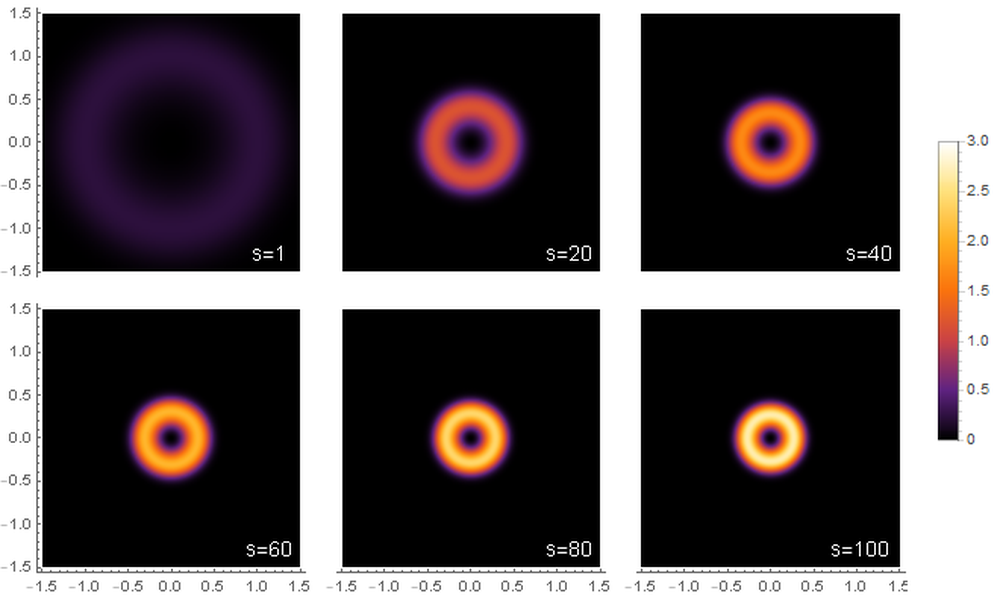
\includegraphics[width=1\textwidth]{sp_plane.png}
	\caption{Density plot of the absolute value squared of \eqref{eq_plane_spf_evolution} for different values of $s$ plotted as a function of $x$ and $y$.}
	\label{fig_spf_plane_evolution}
\end{figure}

\begin{figure}[htbp]
	\centering
	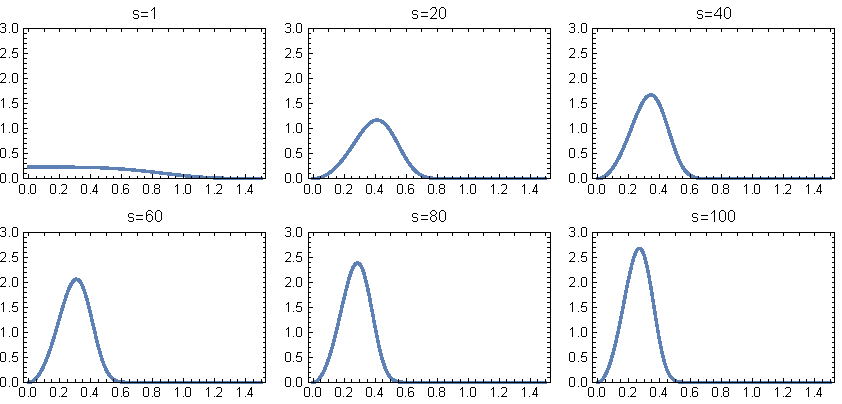
\includegraphics[width=1\textwidth]{sp_plane_section.pdf}
	\caption{Absolute value squared of \eqref{eq_plane_spf_evolution} plotted as a function of $u$ for different values of $s$.}
	\label{fig_spf_plane_evolution_sec}
\end{figure}

For the integer quantum Hall effect, the result is similar. Disregarding the half-form correction in order to simplify the calculations, the integer quantum Hall wave function for $N$ electrons is as in \eqref{eq_integer_wavefunction},
\begin{align} \label{eq_plane_iqh_evolution}
	\psi_{IQHE} = \prod_{1 \leq k<j \leq N}(z_k - z_j) e^{-\frac{\sum_{k=1}^N \abs{z_k}^2}{4}},
\end{align}
and
\begin{align*}
	U_{s,1} \cdot \psi_{IQHE} &\sim e^{-\frac{s}{2}} \prod_{1 \leq k<j \leq N}((z_s)_j - (z_s)_k) e^{-\kpot_s} \\
	&\sim \prod_{1 \leq k<j \leq N}((z_s)_j - (z_s)_k) e^{-\kpot_s}.
\end{align*}
The Laughlin state, although similar to the IQHE state, behaves in a fundamentally different way under time-evolution. It has the expression \eqref{eq_laughlin_wavefunction}
\begin{align*}
	\psi_\text{L} \sim \prod_{1 \leq k < j \leq N}(z_j - z_k)^m e^{\frac{-\sum_{k=1}^N \abs{z_k}^2}{4}}.
\end{align*}
Applying the GCST, we obtain
\begin{align*} U_{s,1}(\Psi_{L}) \sim e^{-s\widehat\qs(H)} \left ( \prod_{1 \leq k < j \leq N}^N((z_{s})_j - (z_{s})_k)^m e^{-\kpot_s}\right ).
\end{align*}
The operator $e^{-s\q{H}}$ fundamentally changes the wave function. For example, for two particles and no quasiholes,
\begin{align}
&e^{\frac{s}{2}\left (\frac{\partial^2}{\partial \theta_1^2} + \frac{\partial^2}{\partial \theta_2^2} \right )} \cdot \left [ ((z_1)_{s} - (z_2)_{s})^3 \right ] \nonumber \\
=& \left ( e^{-\frac{9}{2}s} (z_1)_{s}^3 - 3 e^{-\frac{5}{2}s} (z_1)^2_{s}(z_2)_{s} +  3 e^{-\frac{5}{2}s} (z_1)_{s}(z_2)^2_{s} + e^{-\frac{9}{2}s} (z_2)_{s}^3\right ) \label{eq_prefactor_change_plane} \\
\not\sim& ((z_1)_{s} - (z_2)_{s})^3. \nonumber
\end{align}
Considering now the wave function in the presence of $R$ quasiholes, as in \eqref{eq_laughlin_wavefunction_qh}, and its time-evolution,
\begin{align*}
	\psi_\text{L,QH} &\sim \prod_{j = 1}^{N}\prod_{k = 1}^{R}(z_j - \nu_k) \prod_{1 \leq k < j \leq N}(z_j - z_k)^m e^{-\kpot} \\
	U_{s,1} \psi_\text{L,QH} &\sim e^{-s\q{H}} \left ( \prod_{j = 1}^{N}\prod_{k = 1}^{R}((z_{s})_j - \nu_k) \prod_{1 \leq k < j \leq N}((z_{s})_j - (z_{s})_k)^m e^{-\kpot_s}\right ),
\end{align*}
the quasihole factors also suffer a change. Indeed, a factor of $e^{-\frac{s}{2}}$ appears on the time-evolved complex variable $z_{s}$ with no compensating factor for the corresponding quasihole term:
\begin{align} \label{eq_qh_change}
U_{s,1}(z_j - \nu_k) &= e^{-\frac{s}{2}}(z_j)_{s} - \nu_k \\
&\sim (z_j)_{s} - e^{\frac{s}{2}}\nu_k .\nonumber
\end{align}

In the case of the Moore-Read state, as in \eqref{eq_mr_wavefunction}, 
\begin{align}
	\Psi_{\text{MR}} =  \Pf\left ( \frac{1}{z_k - z_j} \right ) \prod_{1 \leq k < j \leq N}^N(z_j - z_k)^m e^{-\kpot},
\end{align}
we obtain
\begin{align} \label{mr_evolved}
	U_{s,1}(\Psi_{\text{MR}}) = e^{-s\q{H}} \left ( \Pf\left ( \frac{1}{(z_{s})_j - (z_{s})_k} \right ) \prod_{j > k}^N((z_{s})_j - (z_{s})_k)^m e^{-\kpot_s}\right ).
\end{align}
By applying $e^{- \widehat \qs(H)}$, the polynomial structure becomes even less uniform since some cancellation with the Pfaffian factor happens. For example, for four particles,
\begin{align*}
	\Pf\left ( \frac{1}{z_k - z_j} \right )  = \frac{1}{z_1 - z_2}\frac{1}{z_3 - z_4} - \frac{1}{z_1 - z_3}\frac{1}{z_2 - z_4} + \frac{1}{z_1 - z_4} \frac{1}{z_2 - z_3},
\end{align*}
and so, for instance, assuming $m=2$ and expanding the Pfaffian as above, the holomorphic prefactor has a term
\begin{align} \label{eq_pfaffian_structure_change}
	p = (z_1 - z_2)(z_1 - z_3)^2(z_1 - z_4)^2(z_2 - z_3)^2(z_2 - z_4)^2(z_3 - z_4),
\end{align}
which means that when we apply $e^{- \widehat \qs(H)}$ to the above expression and distribute it using the Leibniz rule, it will act on factors having different powers, resulting in two terms which are proportional to $p$ and four terms which have a factor of the form $\left ( e^{-2s} (z_k)_{s}^2 - 2 e^{-s} (z_k)_{s}(z_j)_{s} + e^{-2s} (z_j)_{s}^2\right )$. 

\section{Evolution on a deformed cylinder with $S^1$-symmetry} \label{sec_cyl}
Here, our Riemann surface will be the infinite cylinder $\mfld = \reals \times S^1$ with standard symplectic structure and the standard complex structure as the initial complex structure.

We consider the Kähler toric action given by a rotation of the cylinder along its axis
\begin{align*}
	\tact: S^1 \times (\reals \times S^1) &\to (\reals \times S^1) \\
	(e^{it}, (u,\theta)) &\mapsto (u, \theta + t).
\end{align*}
This action has moment map
\begin{align*}
	\mmap: \reals \times S^1 &\to \reals \\
	(u, \theta) &\mapsto u
\end{align*}
and it is such that $\mfld^\circ = \mfld$. It is clear that $(u, \theta)$ as above define action-angle coordinates. Note that these also define a toric holomorphic chart $z = v + i\theta$ with $v = u$.

Choose the initial Kähler potential $\kpot_0 = \frac{u^2}{2}$, which coincides with the initial symplectic potential $\sgen_0$ in this case. Recalling point \eqref{intro_symplectic_evolution}, we obtain
\begin{align*}
	g_{s} = \frac{u^2}{2} + sH.
\end{align*}

% Note also from \eqref{eq_plane_ktoric_evolution} that the action of the complex time flow on the usual complex coordinate is
% \begin{align} \label{eq_plane_normal_evolution}
% 	z_s := \left ( \phi_\tau^{X_H} \right )^* z \big|_{\tau=is} = e^{su}z
% \end{align}

Here, we consider a Hamiltonian $H \in C^\infty(\mfld)$ such that $H'' = e^{-u^2}$, i.e.
\begin{align*}
	H' &= \frac{\sqrt{\pi}}{2}\erf(u), \\
	H &= \frac{1}{2}e^{- u^2} + \frac{\sqrt{\pi}}{2}u\erf{u},
\end{align*}
where $\erf(u) := \frac{2}{\sqrt{\pi}}\int_0^u e^{-t^2} dt$ is the \emph{error function}. This is partially motivated by the deformation (26) of \cite{johri_probing_2016}. From this and the previous considerations we obtain
\begin{align}
	\metric_s &= \left( 1 + se^{-u^2} \right) du^2 + \left( \frac{1}{1+se^{-u^2}} \right) d\theta^2, \\ \nonumber
	\kpot_s &= \frac{u^2}{2} + s (u H' - H), \nonumber \\
	S_s &= - \left( \frac{1}{1+se^{-u^2}} \right)''. \label{eq_cyl_curvature}
\end{align}
\begin{figure}[htbp]
	\centering
	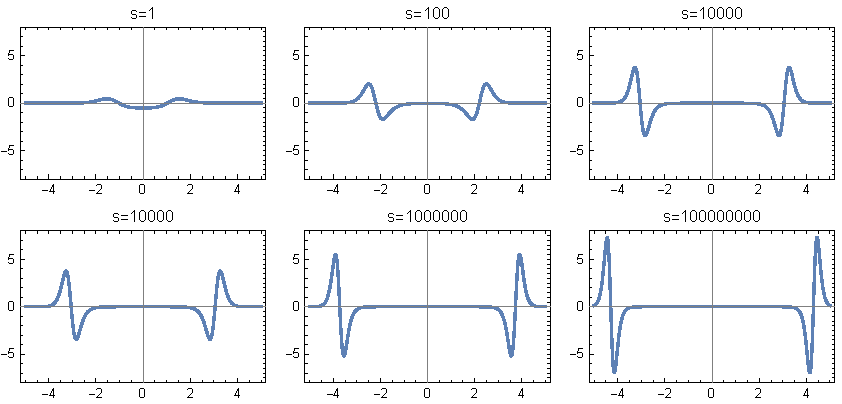
\includegraphics[width=1\textwidth]{cylinder_curvature.pdf}
	\caption{Curvature of cylinder \eqref{eq_cyl_curvature} plotted as a function of $u$.}
	\label{fig_cylinder_curvature}
\end{figure}
\begin{figure}[htbp]
	\centering
	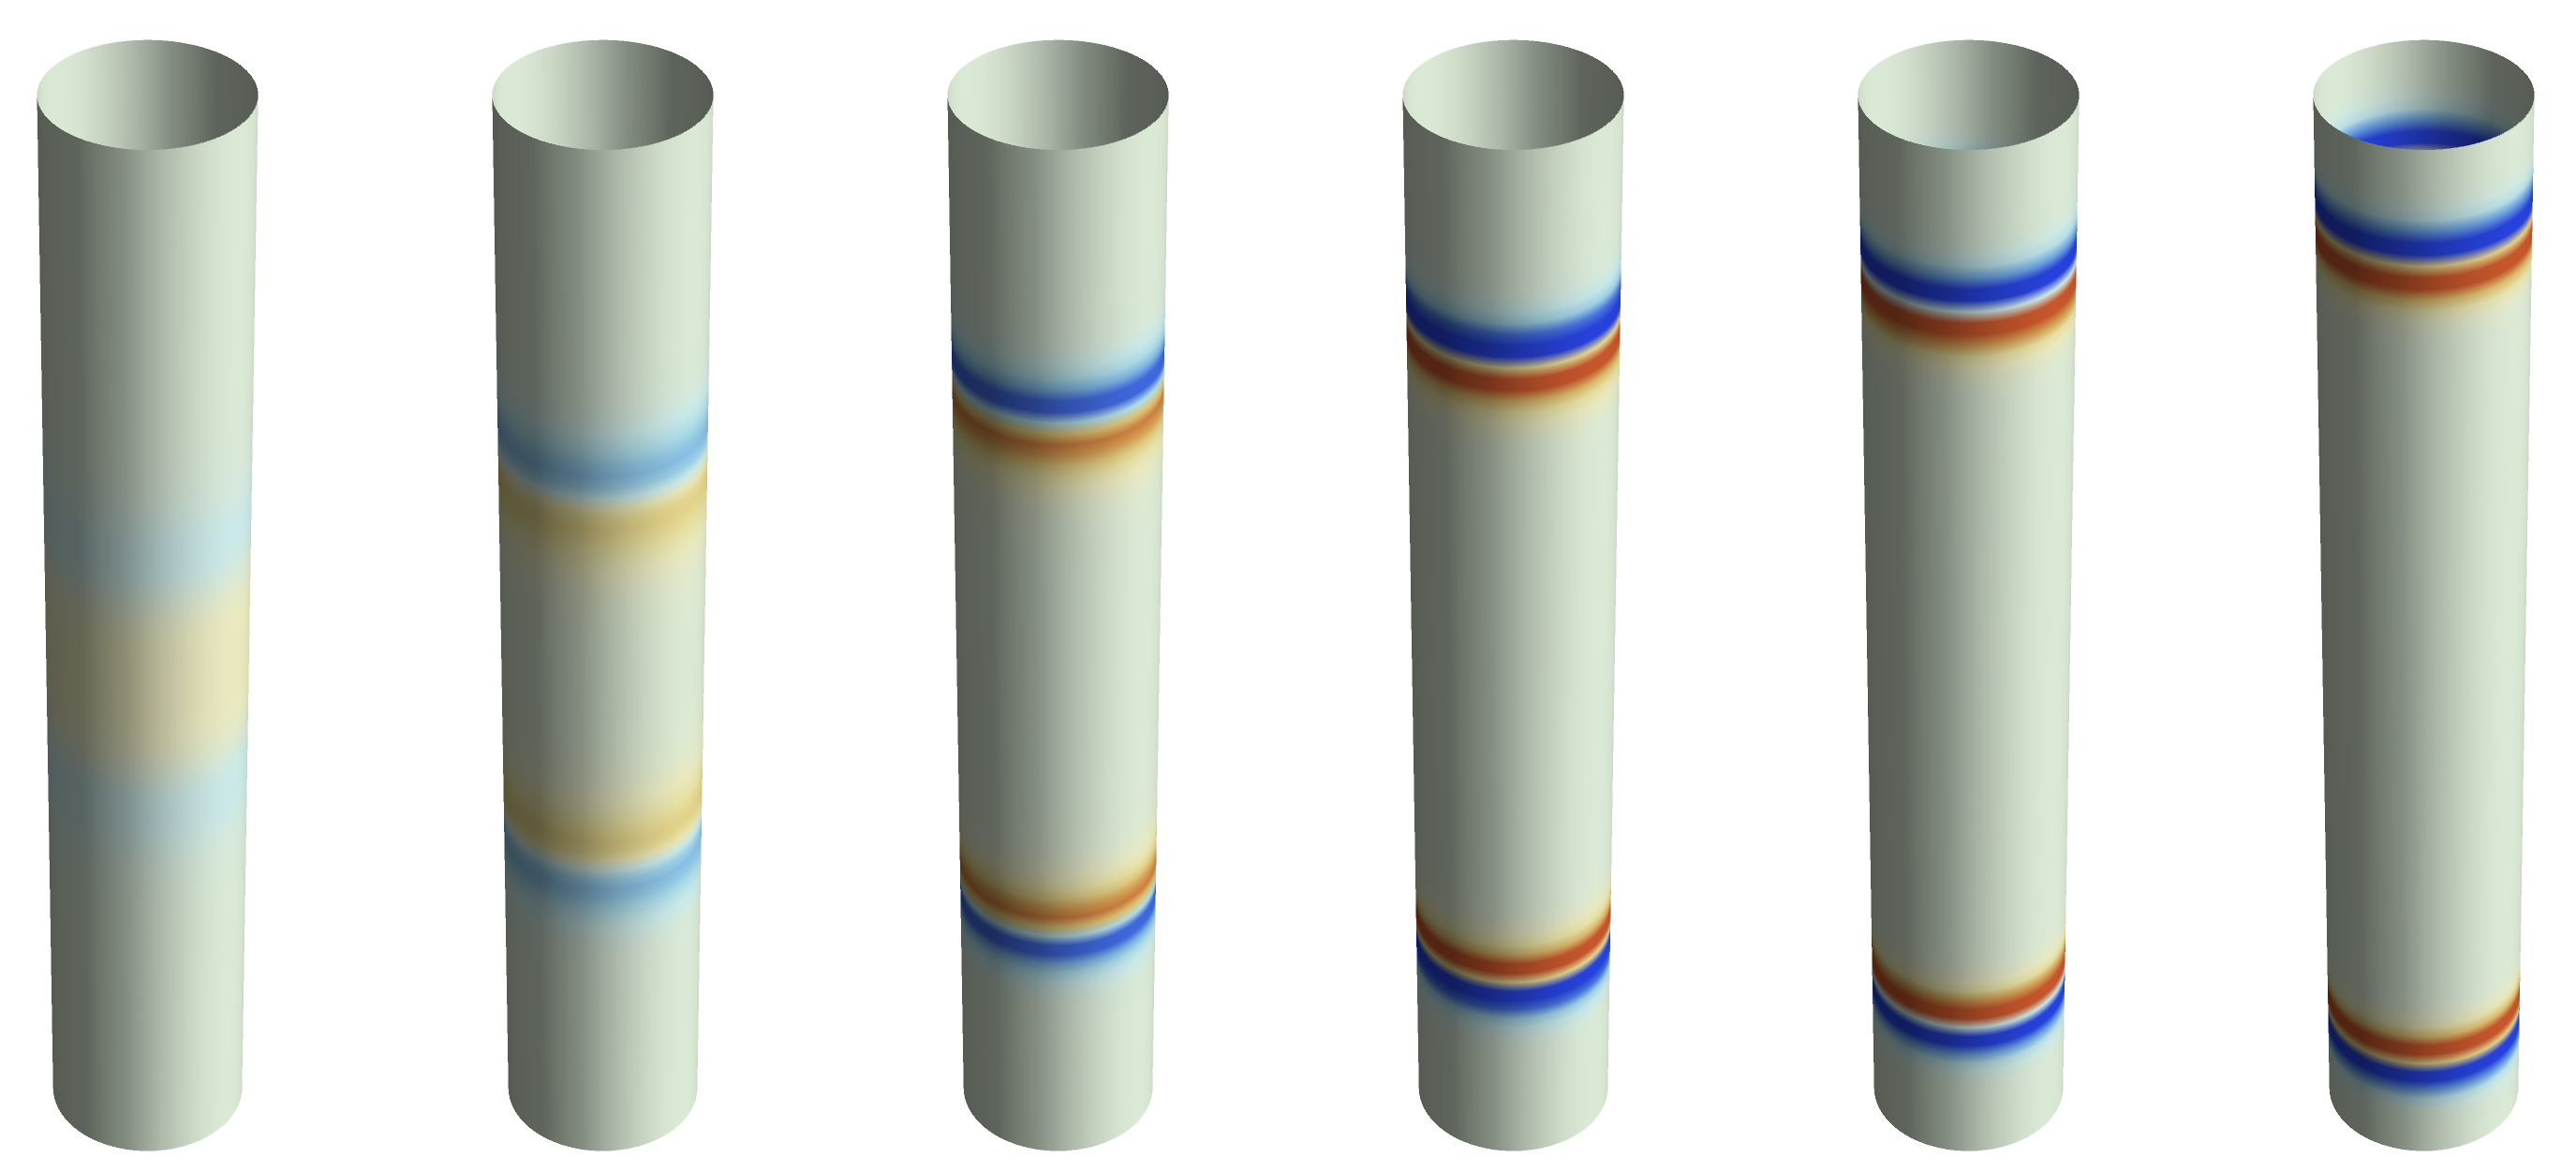
\includegraphics[width=0.8\textwidth]{cylinder_curvature_surface.png}
	\caption{Density plot of the curvature of the cylinder \eqref{eq_cyl_curvature} in three dimensions, for the same values of $s$ as in \figref{fig_cylinder_curvature}.}
	\label{fig_cylinder_curvature_surface}
\end{figure}
\begin{figure}[htbp]
	\centering
	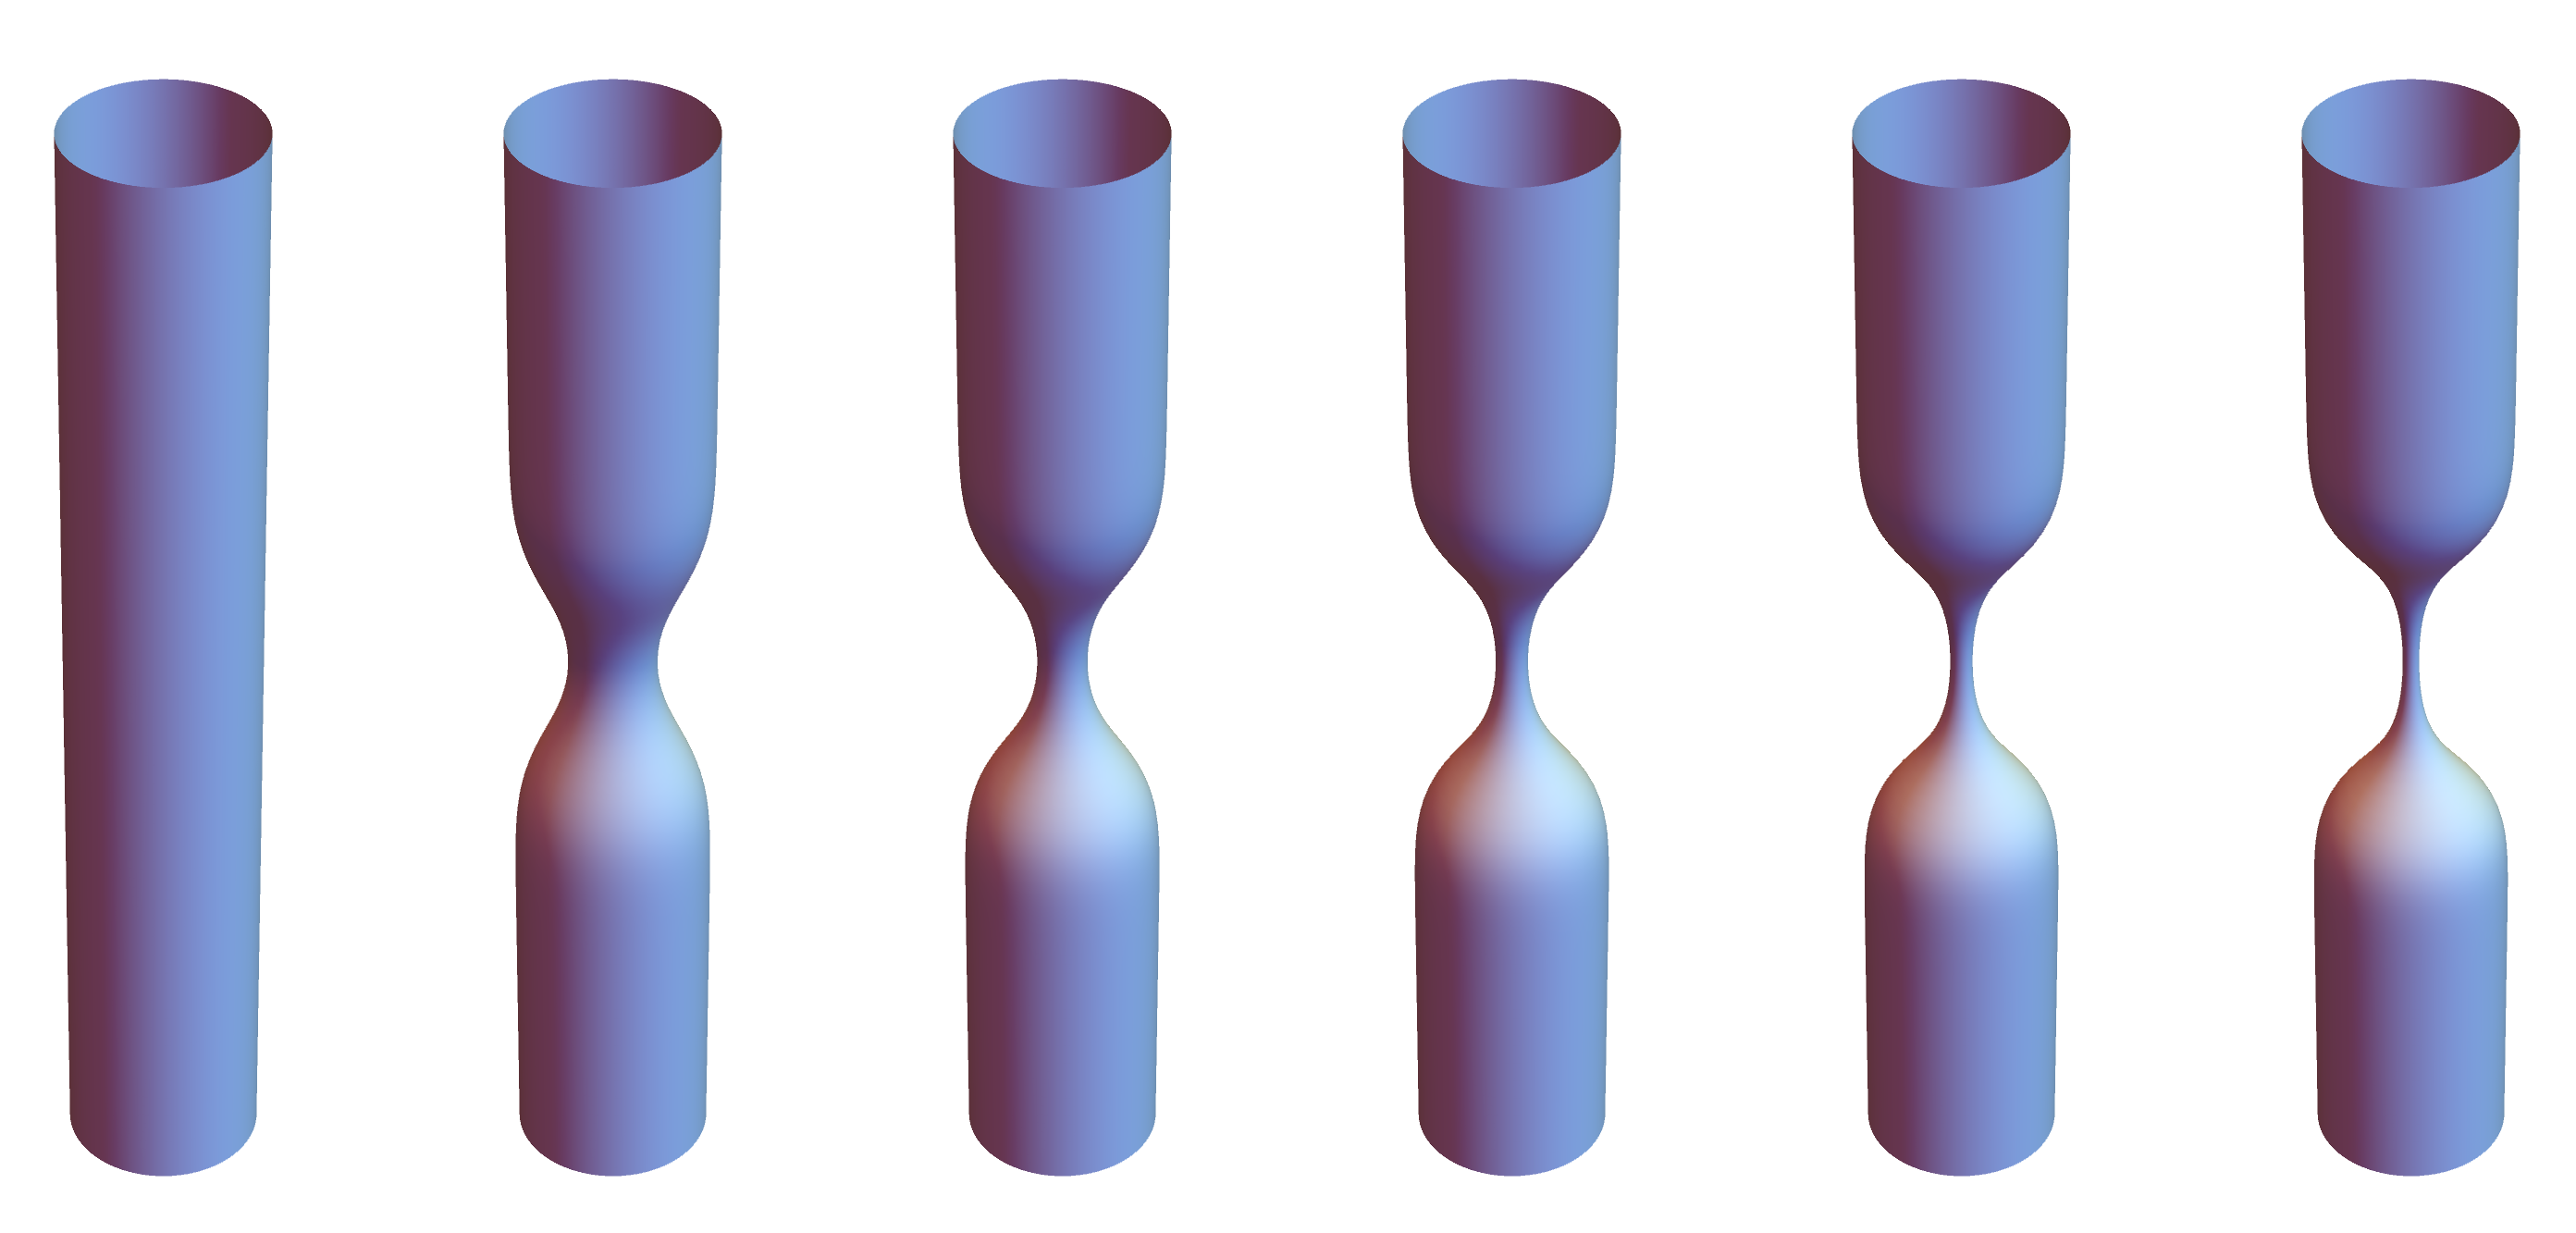
\includegraphics[width=0.8\textwidth]{cylinder_curvature_surface_isometry.png}
	\caption{Three dimensional illustration of the deformation that the cylinder undergoes. For visualization purpoeses, here we are rescaling the metric along the cylinder axis.}
	\label{fig_cylinder_curvature_illustration}
\end{figure}
We extend this to $N \in \nats$ particles. The Riemann surface representing the configuration space of the particles will be the Cartesian product $(\reals \times S^1)^N \cong (\reals^{N} \times \torus^N)$. We consider the trivial complex line bundle, $L = (\reals^{N} \times \torus^N) \times \cmplx$, with $\spot = \sum_{k=1}^{N} u_k d\theta_k$, unitary trivialization $\utriv \equiv 1$, connection $\covd{X} = X + i \spot(X)$ and Hermitian structure $\hip{a}{b} = a \bar{b}$ for $a, b \in C^\infty(\reals^{N} \times \torus^N; \cmplx)$. The square root $\sqrtb_\pol$ of the canonical bundle is trivial with trivializing section represented by $\sqrt{dz_1 \wedge ... \wedge dz_N}$. The polarization $\pol_0$ comes from the complex structure i.e. $\overline \pol_0$ is spanned by $\{\pd{\bar z_k}\}_{k=1,...,N}$, and the time-evolved polarization $\pol_\tau$ is such that $\overline \pol_\tau$ is spanned by $\{\pd{ (\bar z_{s})_k}\}_{k=1,...N}$, where $(z_{s})_k = \left ( \phi_{\tau}^{X_H} \right )^* z_k \big|_{\tau=is}$ and $\bm{H} = \sum_{k=1}^{N} \frac{1}{2}e^{- u_k^2} + \frac{\sqrt{\pi}}{2}u_k\erf{u_k}$. 

In order to write the GCST associated to $\bm{H}$, we first determine the prequantizations and quantizations of the relevant observables. 

\begin{align*}
	\prqs_1(\bm{H}) &= \sum_{k=1}^{N} - i \hbar H_k' \pd{\theta_k} - u H_k' + H_k, \\
	\prqs_2(\bm{H}) &= i \sum_{k=1}^{N} \lied{\left( - H_k' \pd{\theta_k} \right)}, \nonumber\\
	\qs_1(\bm{H}) &= \sum_{k=1}^{N} H_k \left (- i \pd{\theta_k} \right ), \nonumber \\
	\qs_2(\bm{H}) &= \sum_{k=1}^{N} H_k \left (\lied{-\pd{\theta_k}} \right ) . \nonumber
\end{align*}
\begin{align*}
	U_{s,1} &=  e^{ \sum_{k=1}^{N} -siH_k'\pd{\theta_k}-suH_k'+sH_k} \circ e^{ \sum_{k=1}^{N} -sH_k(-i  \pd{\theta_k})}, \\
	U_{s,2} &=  e^{i \sum_{k=1}^{N} \lied{\left( - u_k \pd{\theta_k} \right)}} \circ e^{ \sum_{k=1}^{N} H_k \left (\lied{-\pd{\theta_k}} \right )}
\end{align*}
We will work with adaptations of the quantum Hall states for the cylinder given in \cite{azuma_explicit_1994}. The wave function for one particle in the LLL takes the form
\begin{align*}
	\psi_{m} &\sim \tilde \psi_m \otimes \sqrt{dz},
\end{align*}
where
\begin{align*}
	\tilde \psi_{m} &\sim w^m e^{-\kpot_0} = e^{2 \pi m (u + i\theta)} e^{-\frac{u^2}{2}}
\end{align*}
and $w = e^{m 2\pi (u+i\theta)}$. Applying the GCST, we obtain
\begin{align}\label{eq_cyl_spf_evolution}
	U_{s,1} \tilde \psi_m &= e^{-s H \left (2 \pi m \right )}e^{ms H'(u) 2\pi}e^{-s(u H' - H)} e^{m 2\pi (u_k+i\theta_k)} e^{-\frac{u^2}{2}} \nonumber \\
	&= e^{-s H \left (2 \pi m \right )}e^{ms H'(u) 2\pi}e^{m 2\pi (u_k+i\theta_k)} e^{-\kpot_s} \\
	&= e^{-s H \left (2 \pi m \right )} w_s e^{-\kpot_s}, \nonumber
\end{align}
where $w_s = e^{\frac{2\pi \left (v_s + i \theta \right )}{L_x}}$, and
\begin{align*}
	U_{s,2} \cdot \sqrt{dz} &= e^{i s\lied{-u \pd{\theta}} } \cdot \sqrt{dz} \\
	&= \sqrt{dv + i \, d \left( 1 - i s H' \pd{\theta} \right)\theta}\\
	&= \sqrt{dv + i d \theta + s dH'} \\
	&= \sqrt{dv_{s} + i d \theta} \\
	&= \sqrt{dz_{s}}
\end{align*}
\begin{figure}[htbp]
	\centering
	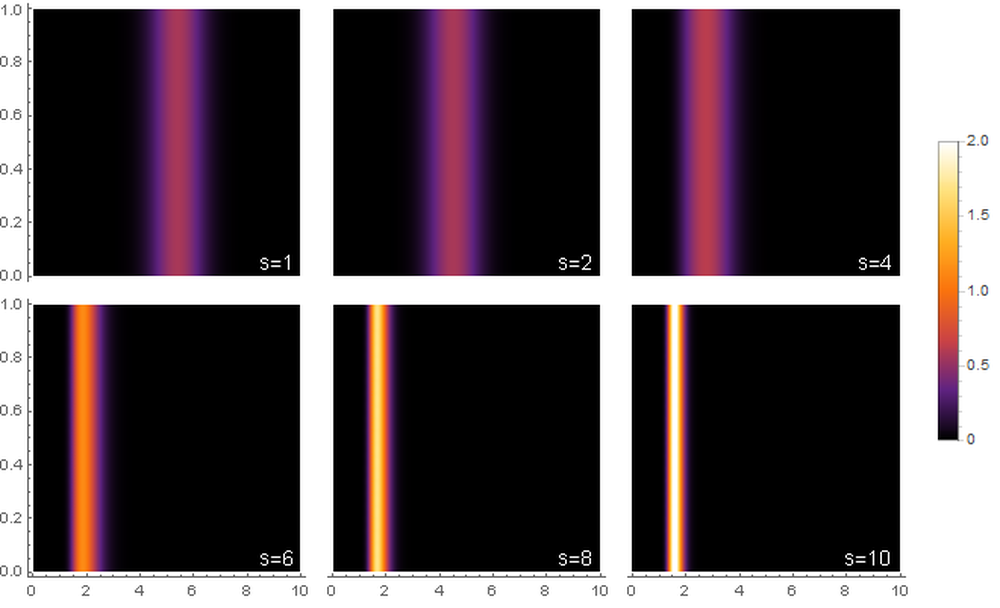
\includegraphics[width=1\textwidth]{sp_cyl.png}
	\caption{Density plot of the absolute value squared of \eqref{eq_cyl_spf_evolution} for different values of $s$.}
	\label{fig_spf_cyl_evolution}
\end{figure}
\begin{figure}[htbp]
	\centering
	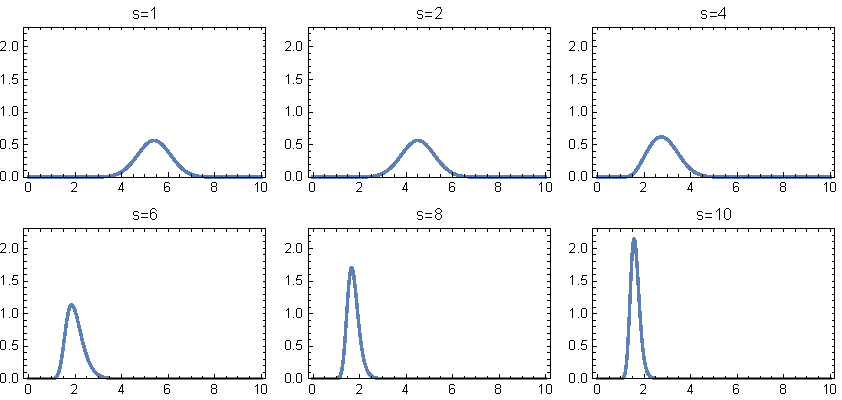
\includegraphics[width=1\textwidth]{sp_cyl_section.pdf}
	\caption{Absolute value squared of \eqref{eq_cyl_spf_evolution} plotted as a function of $u$ for different values of $s$.}
	\label{fig_spf_cyl_evolution_sec}
\end{figure}
In order to simplify the calculations, we will not consider the half-form correction in the remainder of this section. The wave function for the fully filled LLL is
\begin{align*}
	\psi_\text{IQHE} = \prod_{1 \leq k < j \leq N}(w_j-w_k) e^{-\sum_{k}\frac{u_k^2}{2}} &= \prod_{1 \leq k < j \leq N}\left(e^{2\pi (u_j + i \theta_j)}-e^{2\pi (u_k + i \theta_k)}\right) e^{-\sum_{k}\frac{u_k^2}{2}},
\end{align*}
where $w_k = e^{2\pi (u_k+i\theta_k)}$. Applying the GCST, we obtain
\begin{align} \label{eq_cyl_iqh_evolution}
	U_{s,1} \psi_\text{IQHE} = \prod_{1 \leq k < j \leq N}((w_j)_s-(w_k)_s) e^{-\kpot_s},
\end{align}
where $(w_k)_s = e^{2\pi \left ((v_k)_s + i \theta_k \right )}$. 

The Laughlin wave function for the case of the cylinder is
\begin{align} \label{eq_laughlin_cyl}
	\psi_\text{L} = \prod_{1 \leq k < j \leq N}(w_j-w_k)^m e^{\left( -\sum_{k}\frac{u_k^2}{2}\right)} &= \prod_{1 \leq k < j \leq N}\left(e^{2\pi (u_j + i \theta_j)}-e^{2\pi (u_k + i \theta_k))}\right)^m e^{\left( -\sum_{k}\frac{u_k^2}{2}\right)}
\end{align}
and, applying the GCST, the structure of the holomorphic factor of the wave function is fundamentally changed, as in the case of the plane 
\begin{align*}
	U_{s,1} \psi_\text{L} = e^{- s \sum_{k=1}^{N} H_k \left (- i \pd{\theta} \right )} \cdot \left ( \prod_{1 \leq k < j \leq N}(w_j-w_k)^m e^{\left( -\sum_{k}\frac{u_k^2}{2}\right)} \right )
\end{align*}
\begin{align}
	&e^{- s \sum_{k=1}^{N} H_k \left (- i \pd{\theta} \right )} \cdot \left [ ((w_1)_{s} - (w_2)_{s})^3 \right ] \nonumber \\
	&=  e^{-s H \left (3 \cdot 2 \pi \right )} (w_1)_{s}^3 - 3  e^{-s H \left (2 \cdot 2 \pi \right ) + H \left (2 \pi \right )} (w_1)^2_{s}(w_2)_{s} \label{eq_prefactor_change_cyl}\\ 
	&- 3 e^{-s H \left (2 \pi \right ) + H \left (2 \cdot 2 \pi \right )} (w_1)_{s}(w_2)^2_{s} + e^{-s H \left (3 \cdot 2 \pi \right )} (w_2)_{s}^3 \nonumber \\
	&\not\sim ((w_1)_{s} - (w_2)_{s})^3. \nonumber
\end{align}

For simplicity, we do not consider quasiholes or the Moore-Read state for the cylinder.

We now examine what happens to the wave function for a particle in the LLL on the cylinder when one takes the limit $s \to \infty$.
\begin{prop}
Let $(\mfld,\sform,\cstruct_0,\hact)$ be a Kähler toric manifold with action-angle coordinates $(u,\theta)$ defined on $\mfld^\circ$. Pick an $S^1$-invariant Hamiltonian $H \in C^\ra(\mfld)$ and consider $P_s = (\phi_{is})^* P_0$ as in \eqref{eq_evolved_pol} assuming no convergence problems for $s \in \reals^+$. Then
	\begin{align*}
		\lim_{s \to \infty} \pol_s =  \langle X_u \rangle = \left \langle \pd{\theta} \right \rangle,
	\end{align*}
	where $\langle \cdot \rangle$ denotes the linear span of the elements enclosed by the brackets.
\end{prop}
\begin{proof}
	Using \eqref{eq_cylinder_ktoric_evolution},
	\begin{align*}
		\pol_s &= \langle X_{z_s} \rangle = \langle X_u + s X_{H'(u)} + i X_\theta \rangle \\
		&= \left \langle - H''(u) \pd{\theta} + \frac{1}{s}(X_u + i X_\theta) \right \rangle \to_{s \to \infty} \left \langle \pd{\theta} \right \rangle.
	\end{align*}
\end{proof}
% \begin{align*}
% 	f(x_0) &= \lim_{a \to 0} \int_\reals \frac{e^{-\frac{(u-u_0)^2}{2a}}}{\sqrt{2 \pi a}}du f(u)
% \end{align*}
Now, adapting the proof of Lemma 3.7 of \cite{baier_toric_2011}, we obtain that 
% following result.
% \begin{thm}
	
% 	\begin{align*}
% 		\int_\reals A_s \sqrt{s}e^{fs} dz = 1 \forall s > 0
% 	\end{align*}
% 	$f$ convex with a global minimum at $x_0$. Then
% 	\begin{align*}
% 		\lim_{s\to\infty}A_s &= a_\infty \in ]0,\infty[ \\
% 		\lim_{s \to \infty} A_s \sqrt{s}e^{-fs}&=\delta(x-x_0)
% 	\end{align*}
% 	\begin{align*}
% 			\delta(u - u_0) &= \lim_{a \to 0} e^{-\frac{(x-x_0)^2}{2a}}\frac{1}{\sqrt{2\pi a}} dx \\
% 	\end{align*}
% \end{thm}

% From the previous theorems, we get that
\begin{align*} \label{eq_cyl_limit}
	\tilde \psi_m &= e^{-s(\tilde k_m + H(2 \pi m))}w^m e^{-\kpot} \sqrt{s(H''(u)du+\frac{1}{s}(du + i d\theta))} \\
	&\xrightarrow{s\to\infty} ~ \delta(u-2\pi m) e^{2 \pi m + 2 \pi m i \theta} \sqrt{H''(2\pi m)}\sqrt{du}, \nonumber
\end{align*}
yielding a distributional wave function.


% \section{Deformed torus}
% \cite{gradshtein_table_2007} odd theta function
% \begin{align*}
% 	z_{it} &= e^{itX_f}z = x+itf'(y)+iy \\
% 	&= x+i(y+tf'(y))
% \end{align*}
% \begin{align*}
% 	\vartheta(z) = \frac{1}{i}\sum_{n=-\infty}^{\infty}(-1)^n q^{\left(n+\frac{1}{2}\right)^2}e^{(2n+1)zi} = 2\sum_{n=1}^{\infty}(-1)^{n+1}q^{\left(n-\frac{1}{2}\right)^2}\sin[(2n-1)z]
% \end{align*}
% $q=e^{i\pi\tau}$
% wave function \cite{haldane_periodic_1985}
% \begin{align*}
% 	\psi(x,y) &= e^{ikz} e^{-\frac{y^2}{2}} \prod_{\nu=1}^{N}\vartheta\left(  \frac{\pi(z-z_\nu)}{L_1}\Big|\tau\right) \\
% 	&= 2 e^{ikz} e^{-\frac{y^2}{2}} \prod_{\nu=1}^{N} \sum_{n=1}^{\infty}(-1)^{n+1}e^{i\pi\tau\left(n-\frac{1}{2}\right)^2}\sin\left[(2n-1)\frac{\pi(z-z_\nu)}{L_1}\right] 
% \end{align*}
% From \cite{jain_composite_2007}
% \begin{align*}
% 	\psi_{k_x}=\sum_{n=-\infty}^{\infty}e^{-\frac{1}{2}(y-nL_y-k_x)^2}e^{i(k_x+nL_y)x}
% \end{align*}
% with Kähler potential
% \begin{align*}
% 	\psi_{k_x}=e^{-\frac{y^2}{2}}\sum_{n=-\infty}^{\infty}e^{-\frac{1}{2}(y-nL_y-k_x)^2}e^{i(k_x+nL_y)x}=\sum_{n=-\infty}^{\infty}e^{-\frac{1}{2}\left[y^2 + (y-nL_y-k_x)^2 \right]}e^{i(k_x+nL_y)x}
% \end{align*}
% \begin{align*}
% 	H_k(y) &= \frac{\sin(2\pi ky)}{(2\pi k)^2} \\
% 	H'_k(y) &= \frac{\cos(2\pi ky)}{2\pi k} \\
% 	H_k'' &= - \sin(2 \pi k y)
% \end{align*}
% \matosc{
% \[
% 	(u,\theta) \sim (v,\theta)
% \]}


% %_______
% \begin{align*}
% 	X_H &= - H'(y)\pd{x} \\
% 	\prq{H} &= - i \hbar X_H - \spot(X_H) + H \\
% 	\spot &= -y dx \\
% 	\prq{H} &= i \hbar H'(y) \pd{x} - y H'(y) + H = i \hbar \frac{\cos(2\pi ky)}{2\pi k} \pd{x} - \left( y \frac{\cos(2\pi k y)}{2\pi k} - \frac{\sin(2\pi k y)}{(2\pi k^2)} \right)\\
% 	\q{H} &= H(\prq{y}) \\
% 	X_y &= - \pd{x} \\
% 	\prq{y} &= i \hbar \pd{x} \\
% 	\q{H} &= H(i \hbar \pd{x}) = \frac{\sin(2\pi i \hbar k \pd{x})}{(2\pi k)^2} \\
% 	U_{is} &= e^{\frac{s}{\hbar}\prq{H}}\circ e^{-\frac{s}{\hbar}\q{H}} \\
% 	&= e^{siH'(y)\pd{x}-\frac{sy}{\hbar}H'(y)+\frac{s}{\hbar}H}\circ e^{-\frac{s}{\hbar}H(i \hbar \pd{x})} \\
% 	&= e^{i s \frac{\cos(2\pi ky)}{2\pi k} \pd{x} - \frac{s}{\hbar} \left( y \frac{\cos(2\pi k y)}{2\pi k} - \frac{\sin(2\pi k y)}{(2\pi k^2)} \right)}e^{- \frac{s}{\hbar}\frac{\sin(2\pi i k \pd{x})}{(2\pi k)^2}} \\
% 	s_n &=  \\
% 	U_{is} s_n &= 
% \end{align*}
% \begin{align*}
% 	e^{\pd{y}} \psi = e^{\pd{y}}\sum_{n=-\infty}^{\infty}e^{-\frac{1}{2}\left[y^2 + (y-nL_y-k_x)^2 \right]}e^{(k_x+nL_y)x} = 
% \end{align*}
%-------
\end{document}